\documentclass{article}

% if you need to pass options to natbib, use, e.g.:
%     \PassOptionsToPackage{numbers, compress}{natbib}
% before loading tackling_climate_workshop_style

% ready for submission
% \usepackage{tackling_climate_workshop_style}

% to compile a preprint version, e.g., for submission to arXiv, add add the
% [preprint] option:
%     \usepackage[preprint]{tackling_climate_workshop_style}

% to compile a camera-ready version, add the [final] option, e.g.:
%     \usepackage[final]{tackling_climate_workshop_style}

% to avoid loading the natbib package, add option nonatbib:
     \usepackage[nonatbib]{tackling_climate_workshop_style}

\usepackage[utf8]{inputenc} % allow utf-8 input
\usepackage[T1]{fontenc}    % use 8-bit T1 fonts
\usepackage{hyperref}       % hyperlinks
\usepackage{url}            % simple URL typesetting
\usepackage{booktabs}       % professional-quality tables
\usepackage{amsfonts}       % blackboard math symbols
\usepackage{nicefrac}       % compact symbols for 1/2, etc.
\usepackage{microtype}      % microtypography
\usepackage{amsmath}
\usepackage{graphicx}
\usepackage{gensymb}

\title{An Inversion Algorithm of Ice Thickness and InSAR Data for
the State of Friction at the Base of the Greenland Ice Sheet}

% The \author macro works with any number of authors. There are two commands
% used to separate the names and addresses of multiple authors: \And and \AND.
%
% Using \And between authors leaves it to LaTeX to determine where to break the
% lines. Using \AND forces a line break at that point. So, if LaTeX puts 3 of 4
% authors names on the first line, and the last on the second line, try using
% \AND instead of \And before the third author name.

\author{%
  David S.~Hippocampus\thanks{Use footnote for providing further information
    about author (webpage, alternative address)---\emph{not} for acknowledging
    funding agencies.} \\
  Department of Computer Science\\
  Cranberry-Lemon University\\
  Pittsburgh, PA 15213 \\
  \texttt{hippo@cs.cranberry-lemon.edu} \\
  % examples of more authors
   \And
   Coauthor \\
   Affiliation \\
   Address \\
   \texttt{email} \\
   \AND
   Coauthor \\
   Affiliation \\
   Address \\
   \texttt{email} \\
  % \And
  % Coauthor \\
  % Affiliation \\
  % Address \\
  % \texttt{email} \\
  % \And
  % Coauthor \\
  % Affiliation \\
  % Address \\
  % \texttt{email} \\
}

\begin{document}

\maketitle

\begin{abstract}
With the advent of climate change and global warming, the Greenland Ice Sheet (GrIS) has been melting at an alarming rate, losing over 215 Gt per yr, and accounting for ~10\% of mean global sea level rise since the 1990s. It is imperative to understand what dynamics are causing this ice loss and influencing ice flow in order to successfully project mass changes of the GrIS and associated sea level rise. Our work applies machine learning, ice thickness data, and horizontal ice velocity measurements from satellite radar data to quantify the forces and distributions of the basal tractions that are holding the GrIS back from flowing into the ocean. Our physics-based pre-processing algorithm extracts relevant features including the $\varepsilon_{xx}$, $\varepsilon_{yy}$, and $\varepsilon_{xy}$ components of the viscous responses caused by forces on the ice, and feeds it into a linear regression model to predict the forces and distributions of basal tractions across the GrIs. The results of this work enhance knowledge of ice flow by uncovering relationships between basal traction, velocity fields, and ice flux, providing a new method of associating ice loss with sea level changes.
\end{abstract}

\section{Introduction}

With the advent of climate change and global warming, ice sheets worldwide have been melting at an alarming rate. The rate of ice mass loss has increased sixfold from 81 billion tons in the 1990’s to 475 billion tons in the 2010s \cite{the_imbie_team_mass_2020}. The largest contributor to global ice loss is the Greenland Ice Sheet (GrIS), losing over 215 Gt per yr, and accounting for ~10\% of mean global sea level rise since the 1990s ~\cite{stocker_climate_2013}. Rising sea levels have a wide array of disastrous impacts, including coastal erosion, storm surges, flooding, disease spread, and habitat loss that will only continue to worsen in a warming climate \cite{pattyn_greenland_2018}. It is imperative to understand what dynamics are causing this ice loss and influencing ice flow in order to successfully project mass changes of the GrIS and associated sea level rise.

Recent advances in satellite remote sensing systems have produced high-resolution measurements and models of the GrIS, making them an ideal tool for studying motion across large ice sheets. Two-pass Interferometric Synthetic Aperture Radar (InSAR) satellites use radar observations from multiple trips over an area of interest to determine surface motion \cite{wild_differential_2019}. In this work, we utilize high resolution InSAR ice velocity measurements, captured by Sentinel-1 satellite imagery operated by the the ESA By inverting the data using a linear regression model, we quantify forces and distributions of basal tractions (ask about strain rates) that are holding the GrIs back from flowing into the ocean. Initial results show significant correlations between InSAR derived flow rates and strain patterns around the coastline of the ice sheet.

\section{Previous Work}

Glaciologists have traditionally classified ice motion as a viscous flow \cite{morland_steady_1980}. This motivated prior researchers at Stony Brook university to use the bedrock and ice elevations of the GrIs derived from ETOPO1 topographical data set to generate a gravitational potential energy (GPE) map across the GrIs. The primary focus of the research was establishing a connection between GPE calculations and the rate of viscous ice flow, and thus the researchers assumed that the ice was moving along a frictionless base. However, the GPE velocity calculations vastly overestimated the speeds of the ice velocities by a thousand-fold compared to the ground truth data from InSAR satellite imagery. Thus, prior work has reinforced the notion that the basal traction's between the ice and the bedrock have a major influence over ice motion and ice velocity rates \cite{maier_basal_2021}. However, these forces have been poorly characterized as they remain buried beneath thousands of feet of ice \cite{maier_basal_2021}.

Our work is motivated by these results, and acts as an extension building on this prior research to capture a relationship between the InSAR derived horizontal velocity rates and the basal tractions of the GrIs in order to gain insight as to the magnitudes and distributions of the forces holding the ice back from flowing into the ocean. Our approach uses a hybrid model: our ground truth velocity data is used to train a linear regression model, and these model coefficients can be fed into a geophysical model to estimate forces of basal tractions that capture relationships between the ice motion and physical variables.

\section{Methods}

\subsubsection{Dataset}
Our data comes from two sources: ETOPO1 and Sentinel-1 radar satellite imagery. ETOPO1 provides topographical ice and bedrock elevation measurements which are used to calculate the thickness of the ice, and then generate gravitational potential energies (GPE) across the entire ice sheet \cite{information_ncei_etopo1_nodate}. Roughly 1800 Sentinel 1 scenes were used and InSAR feature tracking techniques were applied to derive surface horizontal velocity information of the ice \cite{nagler_sentinel-1_2015}. Both global-level datasets were parsed using the geopandas library to focus on the GrIs from 2016-2017. 

Our data vector is also a model too, as it involves the velocity field of the InSAR associated with our GPE model, which predicts very high as the GPE values are four orders higher than the InSAR values.

Our d vector is almost a negative GPE value, which is why our linear regression coefficents are so high.

\subsubsection{Inversion Set Up}

We are modelling the discrepancies between the velocities calculated by the GPE method and the ground values. Our paper is trying to bridge the gap between the two values.


This data is the foundation for our geophysical equation:

$$
\vec{d}=\overline{\overline{G}} m=v_{\text {InSAR}}-v_{GPE}
$$


$\vec{d}$ is our velocity field representing the difference between the InSAR velocities and the GPE velocities. $\overline{\overline{G}}$ is our basis functions representing the vircous thing-sheet responses casued by body-forces on the ice sheet. $m$ is our linear inversion model. Our goal to find best linear combination $\overline{\overline{G}} m$ that predicts $\vec{d}$. After achieving a proper fit, the model coefficients would be able to provide valuable insight to the distributions of basal tractions, and could also be translated to view the strain rates across the GrIs.

To create our design matrix, $\overline{\overline{G}}$ we partitioned Greenland into 1000 grid cells (each with size 2° x 2°) and generated 3 basis functions ($\varepsilon_{xx}$ - Horizontal East and West effective body forces, $\varepsilon_{yy}$ - Horizontal North and South effective body-forces, and $\varepsilon_{xy}$ - Shear effective body-forces) for each cell. Our original experiments used 40 grid cells (each 10° x 10°), and we noticed considerable performance improvements increasing the resolution of our G matrix. Depending on computational computing power available, further reducing the grid cell size is an avenue for further optimizing the fit of the BLANK linear combination.   

\subsubsection{Model}

This is a linear inversion task, where the effective body-forces in one grid cell can have effects on its surrounding cells and beyond. Thus, it requires a regression model. We use Least Squares Regression from the sklearn library, which has shown to perform well in inversion tasks \cite{lines_review_1984}. To further generalize and optimize the overall fit of our model, we also employed regularization methods Ridge and LASSO. Our Loss Function is defined as [INSERT LOSS HERE], with our alpha value range defined as [alpha]. We used the trade-off (L-curve) criterion and the 10-fold generalized cross validation techniques to determine our optimal smoothing parameter. 

\begin{figure}
    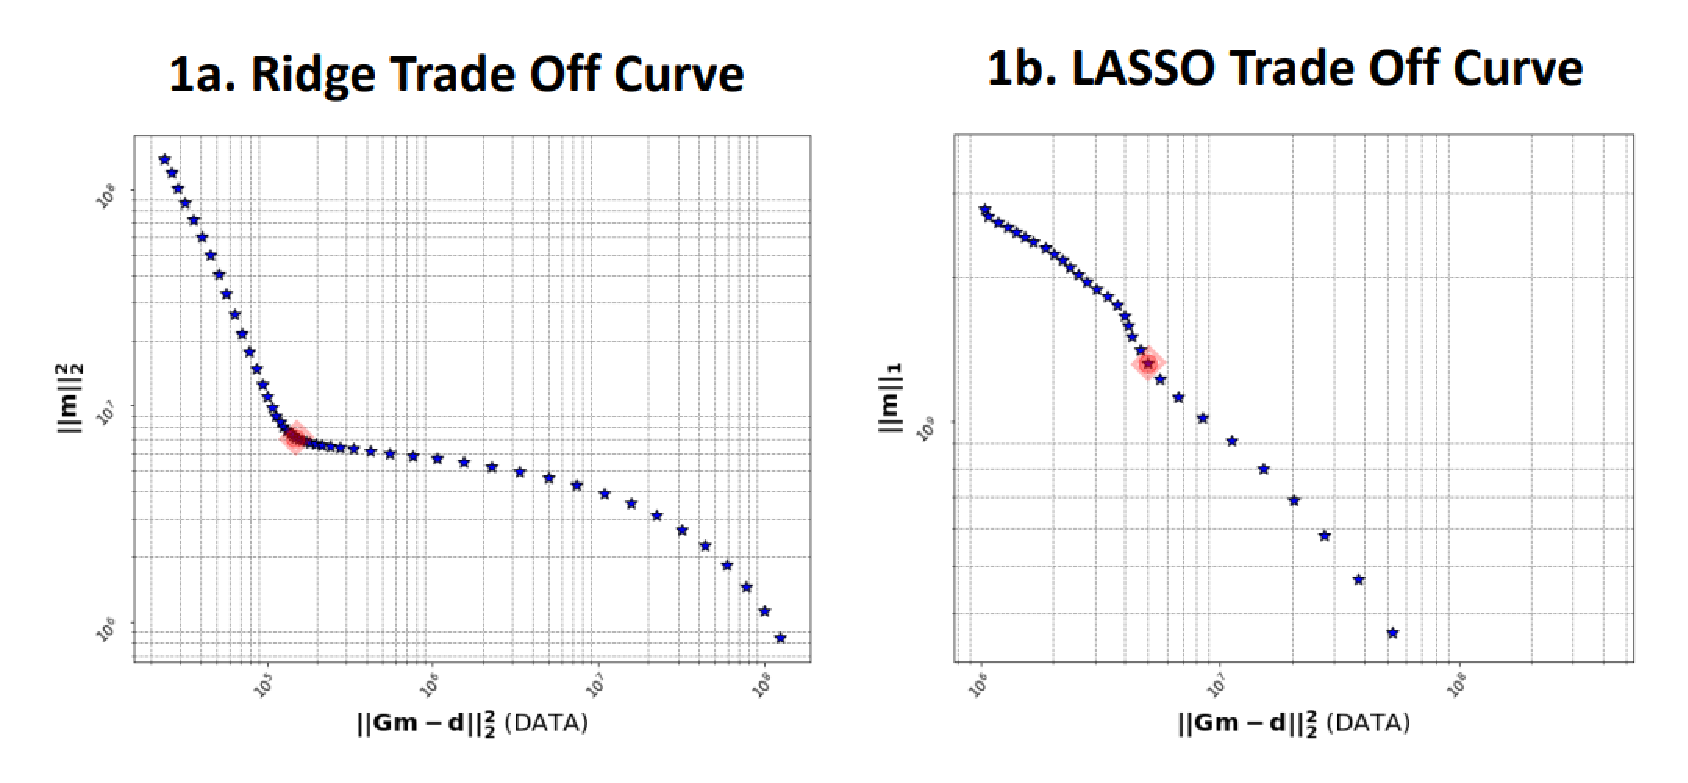
\includegraphics[\columnwidth]{figures/trade-off-curves.pdf}
\end{figure}

\begin{table}
  \caption{Sample table title}
  \label{sample-table}
  \centering
  \begin{tabular}{lll}
    \toprule
    \multicolumn{2}{c}{Part}                   \\
    \cmidrule(r){1-2}
    Name     & Description     & Size ($\mu$m) \\
    \midrule
    Dendrite & Input terminal  & $\sim$100     \\
    Axon     & Output terminal & $\sim$10      \\
    Soma     & Cell body       & up to $10^6$  \\
    \bottomrule
  \end{tabular}
\end{table}

\section{Results}

Both the Ridge and LASSO regression models achieved a near identical fit to the velocity field, achieving $R^{2}$ values of 0.999 and 0.987 respectively. The model predicted plotted against the ground truth velocity field has been shown in Figure BLANK, highlighting the accuracy of the predictions. The slight errors in the predictions seem to be mostly located along the coastline, and we believe that these errors can be corrected for through a smaller grid cell size and access to higher computing power. 



\begin{figure}[!htb]
   \begin{minipage}{0.48\textwidth}
     \centering
     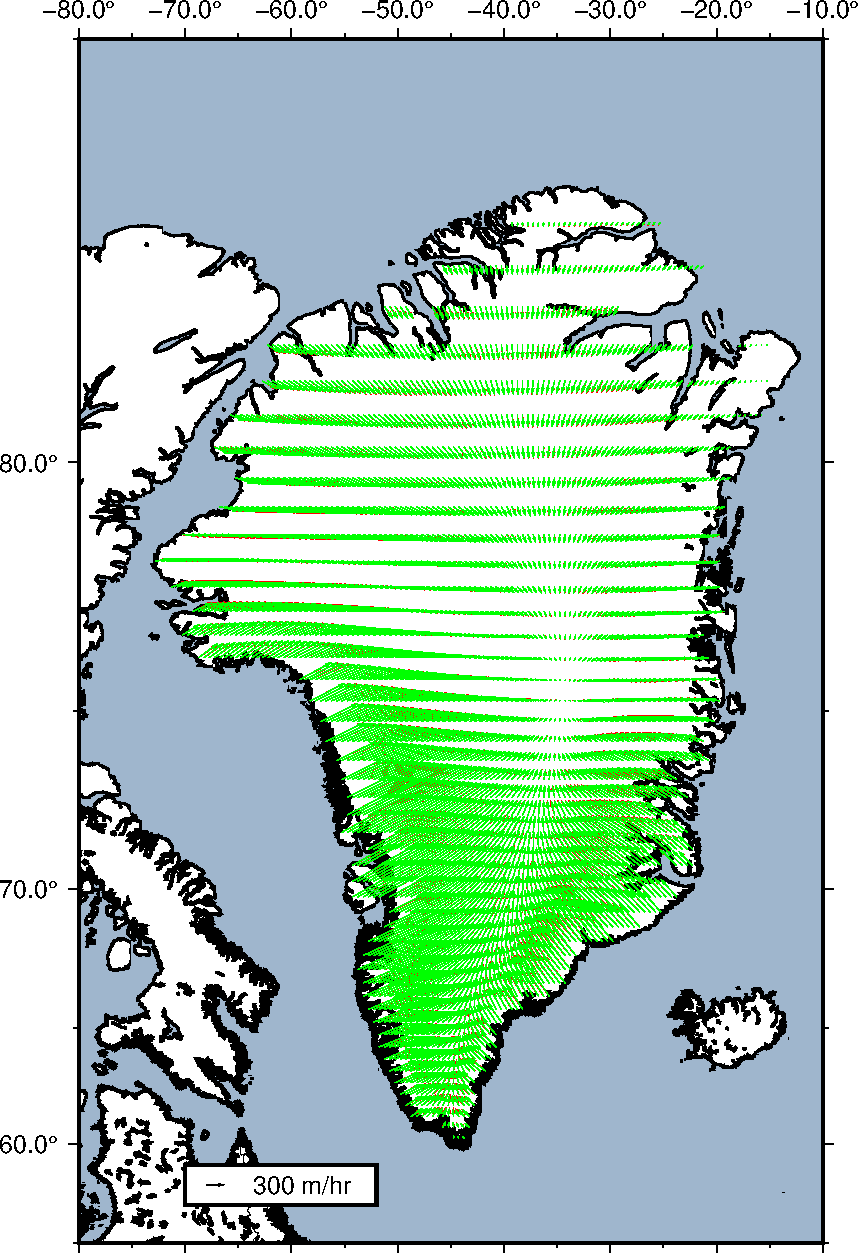
\includegraphics[width=.7\linewidth]{/figures/greenland_inversion_prediction_Ridge_0.15199.pdf}
     \caption{Interpolation for Data 1}\label{Fig:Data1}
   \end{minipage}\hfill
   \begin{minipage}{0.48\textwidth}
     \centering
     \includegraphics[width=.7\linewidth]{example-image-b}
     \caption{Interpolation for Data 2}\label{Fig:Data2}
   \end{minipage}
\end{figure}

\section{Conclusion and Future Work}

In this work, we developed an inversion algorithm for quantifying forces and magnitudes of basal tractions of the Greenland Ice Sheet. This is achieved via a hybrid model, with a linear regression based inversion model that integrates real-world InSAR data, and a physics-based algorithm to predict strain rates from calculated ice velocity fields. This work has large implications on the ability to individually separate basal traction from GPE, and serves as a step towards modeling ice flux in relation to friction, normal forces, and other nonlinear forces. In the future, we hope to use this work to create models relating ice flux in relation to friction, normal forces and nonlinear forces, which would help us relate velocities with ice loss of the GrIs, helping us closely monitor rising sea levels of the GrIs and beyond.


We are currently looking for more data spanning more time or also for the Antarctic Ice Sheet.

REMEMBER TO CTRL F FOR BLANK AT THE END

\bibliography{references}
\bibliographystyle{ieee_fullname}

\end{document}